\chapter{Heaps}
Here, we continue the discussion on queues. 

\section{Introduction}
In some applications, a simple queue may not be the best strategy for completing jobs. Problems arise when small jobs take longer to finish, or important jobs are not processed first.  

That's why we have heaps, which implement a priority queue. Unlike a regular queue, which follows the first-in, first-out (FIFO) principle, a priority queue selects an entry based on specific properties and places it at the front to be processed first.  

For example, in a job queue, various algorithms can be implemented to manage tasks, such as first-come, first-served, shortest-job-first, longest-job-first, priority-based scheduling, or even a combination of these methods.

\subsection{Priority Queue}
A priority queue consists of entries, each containing a key called the priority of the entry. A priority queue supports two primary operations in addition to the usual creation, size, full, and empty checks: \textbf{Insert} and \textbf{Delete\_Min}. Insertion is straightforward, while Delete\_Min finds, returns, and removes the entry with the highest priority. If all entries have equal priorities, the queue follows the FIFO (first-in, first-out) rule.

Several possible implementations include a simple linked list, a sorted contiguous list, an unsorted list, and a binary search tree.

\section{Binary Heaps}
Binary Heaps (or Heaps) have two properties: the \textbf{structure property} and the \textbf{heap order property}. For the \textbf{structure property}, the heap must be a \textbf{complete binary tree}.  

As with AVL trees, an operation on a heap can destroy one of these properties. Therefore, a heap operation must not terminate until all heap properties are restored.  

\subsection{Structure Property}  
A heap is a binary tree that is completely filled (a complete tree), with the possible exception of the bottom level, which is filled from left to right.  

A complete binary tree of height \( h \) has between \( 2^h \) and \( 2^{h+1} - 1 \) nodes. This implies that the height of a complete binary tree is \( \lfloor \log n \rfloor \), which is clearly \( O(\log n) \).  

Because a complete binary tree is so regular, it can be represented in an array, and no pointers are necessary. For example, to represent the tree on the left, we can have:

\begin{minipage}{0.3\textwidth}
\begin{figure}[H]
  \centering
  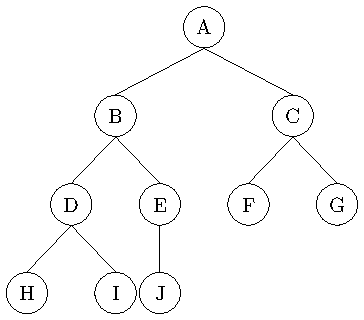
\includegraphics[width=0.75\textwidth]{Figure/Heap1.pdf}
  \caption{Binary Heap}
\end{figure}
\end{minipage}\quad
\begin{minipage}{0.7\textwidth}
\begin{table}[H]
  \centering
  \begin{tabular}{c|c|c|c|c|c|c|c|c|c|c|c|c|c}
    \hline
     & A & B & C & D & E & F & G & H & I & J &  &  &  \\ \hline
    0 & 1 & 2 & 3 & 4 & 5 & 6 & 7 & 8 & 9 & 10 & 11 & 12 & 13 \\
  \end{tabular}
  \caption{Implementation}
\end{table}
\end{minipage}

For any element in array position \(i\), the left child is in position \(2i\), the right child is in the cell after the left child \((2i + 1)\), and the parent is in position \(\left\lfloor \frac{i}{2} \right\rfloor\). Thus, not only are pointers not required, but the operations required to traverse the tree are extremely simple.  

For example, A is in position 1, thus it has no parent. Its children will be in positions \( 2 \) and \( 3 \), which are \( B \) and \( C \). For \( B \) in position 2, its parent will be \( 1 \), which is A. Its children will be in positions \( 4 \) and \( 5 \), which are \( D \) and \( E \).  

The problem is that the estimation of the maximum heap size is required in advance.  

\subsection{Heap Order Property}
This property allows operations to be performed quickly. For a heap, the smallest element should be at the root so that the operation to remove it is efficient. By the heap order property, the minimum element can always be found at the root. Thus, we have the extra operation, find\_min, which can be performed in constant time \(O(1)\).

Since we want to be able to find the minimum quickly, it makes sense that the smallest element should be at the root. If we consider that any subtree should also be a heap, then any node must be smaller than all of its descendants. By applying this logic, we arrive at the heap order property:

In a heap, for every node \(X\), the key in the parent of \(X\) is smaller than or equal to the key in \(X\), except for the root.

\section{Operations}
To perform insertions, we create a hole in the next available location. If \(x\) can be placed in the hole without violating the heap order, then we do so, and the insertion is complete. Otherwise, we slide the element from the parent node of the hole into the hole, thus bubbling the hole up toward the root. We continue this process until \(x\) can be placed in the hole. This strategy is called \textbf{percolate up}.

For example, we use the following method to insert 14 into a heap.
\begin{center}
\begin{minipage}{0.33\textwidth}
\begin{figure}[H]
  \centering
  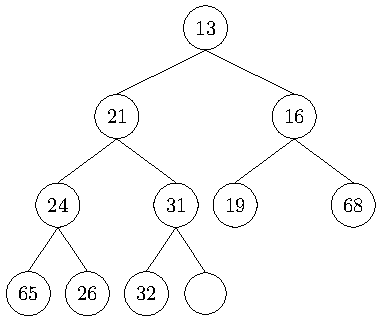
\includegraphics[width=\textwidth]{Figure/HeapI1.pdf}
  \caption{Create hole}
\end{figure}
\end{minipage}
\begin{minipage}{0.33\textwidth}
\begin{figure}[H]
  \centering
  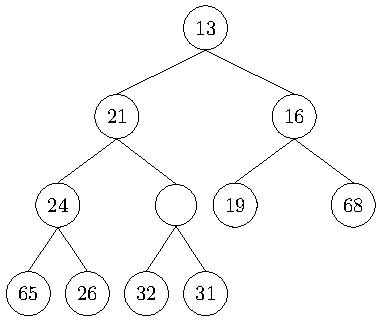
\includegraphics[width=\textwidth]{Figure/HeapI2.pdf}
  \caption{Compare}
\end{figure}
\end{minipage}
\end{center}
\begin{center}
\begin{minipage}{0.33\textwidth}
\begin{figure}[H]
  \centering
  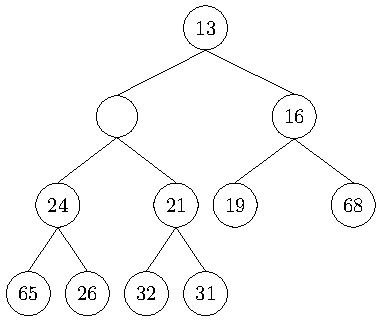
\includegraphics[width=\textwidth]{Figure/HeapI3.pdf}
  \caption{Compare}
\end{figure}
\end{minipage}
\begin{minipage}{0.33\textwidth}
\begin{figure}[H]
  \centering
  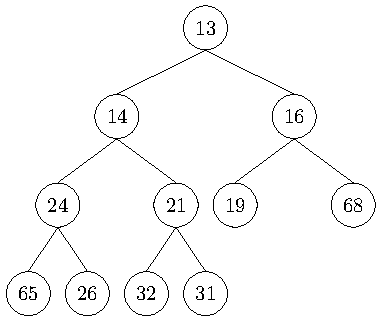
\includegraphics[width=\textwidth]{Figure/HeapI4.pdf}
  \caption{Insert 14}
\end{figure}
\end{minipage}
\end{center}

The time to perform the insertion can be as much as \(O(\log n)\) if the element to be inserted is the new minimum and is percolated all the way to the root. It has been shown before that 2.607 comparisons are required on average to perform an insertion. On average, the insertion moves an element up 1.607 levels.

Deletions are handled in a manner similar to insertions. We only delete from the top since it is the smallest value. When the root is deleted, a hole is created. Then, we slide the smaller of the hole's children into the hole, thus pushing the hole down one level. We repeat this step until \(x\) can be placed in the hole. Thus, our action is to place \(x\) in its correct spot along a path from the root containing the minimum children. The rearranging will typically take less than \(O(\log n)\).

For example, we use the following method to perform deletion:
\begin{center}
\begin{minipage}{0.32\textwidth}
\begin{figure}[H]
  \centering
  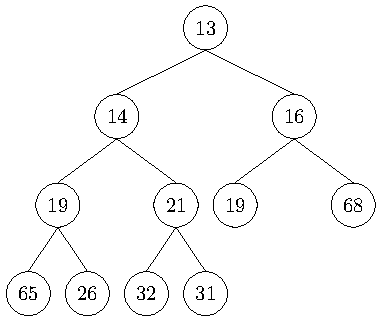
\includegraphics[width=\textwidth]{Figure/HeapD1.pdf}
\end{figure}
\end{minipage}
\begin{minipage}{0.32\textwidth}
\begin{figure}[H]
  \centering
  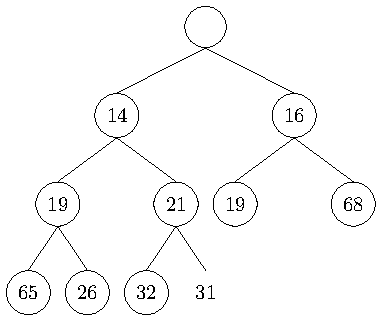
\includegraphics[width=\textwidth]{Figure/HeapD2.pdf}
\end{figure}
\end{minipage}
\begin{minipage}{0.32\textwidth}
\begin{figure}[H]
  \centering
  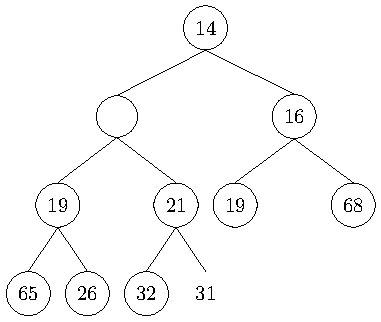
\includegraphics[width=\textwidth]{Figure/HeapD3.pdf}
\end{figure}
\end{minipage}
\end{center}
\begin{center}
\begin{minipage}{0.32\textwidth}
\begin{figure}[H]
  \centering
  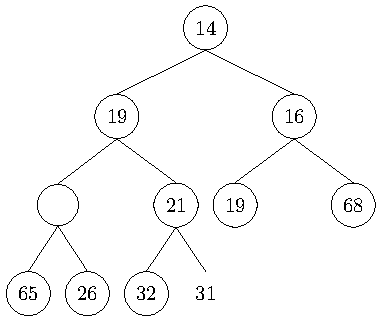
\includegraphics[width=\textwidth]{Figure/HeapD4.pdf}
\end{figure}
\end{minipage}
\begin{minipage}{0.32\textwidth}
\begin{figure}[H]
  \centering
  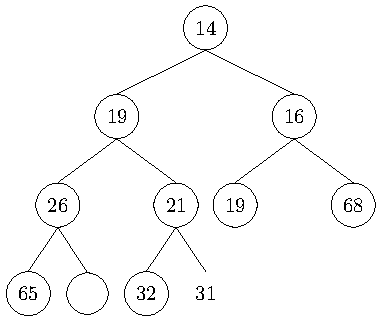
\includegraphics[width=\textwidth]{Figure/HeapD5.pdf}
\end{figure}
\end{minipage}
\begin{minipage}{0.32\textwidth}
\begin{figure}[H]
  \centering
  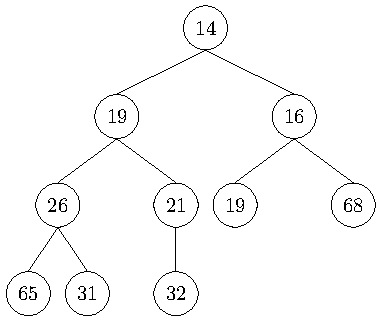
\includegraphics[width=\textwidth]{Figure/HeapD6.pdf}
\end{figure}
\end{minipage}
\end{center}

There are some other heap operations. We can find the minimum in constant time. However, it would be difficult, though possible, to find the maximum, given that there is no ordering information.

To build a heap, we take \(n\) keys and place them into an empty heap. We could then perform \(n\) successive inserts. This will take \(O(n)\) on average but \(O(n \log n)\) in the worst case. Another way is to place the \(n\) keys into the tree in any order, then perform percolate-down on half of the nodes. For example, to insert 15 keys, we can perform percolate-down starting from the 7th node.

\begin{center}
\begin{minipage}{0.24\textwidth}
\begin{figure}[H]
  \centering
  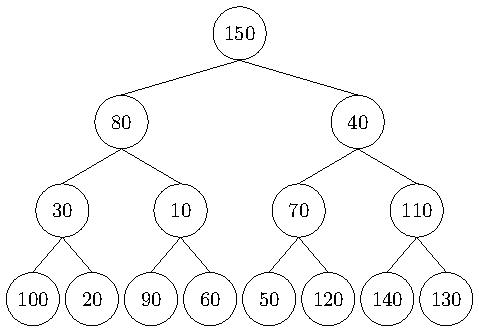
\includegraphics[width=\textwidth]{Figure/Percolate1.pdf}
\end{figure}
\end{minipage}
\begin{minipage}{0.24\textwidth}
\begin{figure}[H]
  \centering
  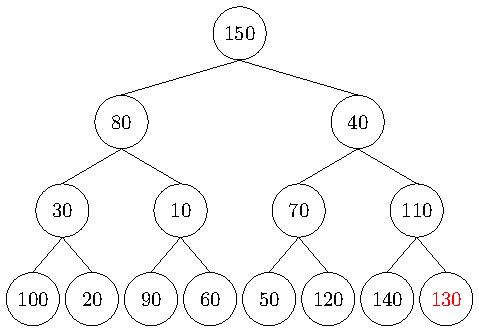
\includegraphics[width=\textwidth]{Figure/Percolate2.pdf}
\end{figure}
\end{minipage}
\begin{minipage}{0.24\textwidth}
\begin{figure}[H]
  \centering
  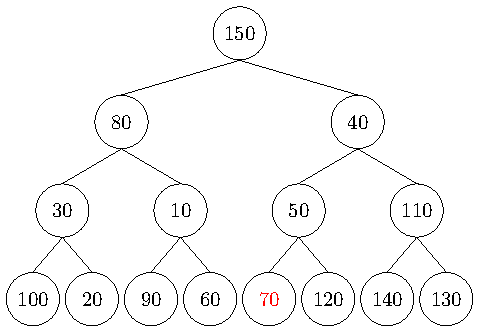
\includegraphics[width=\textwidth]{Figure/Percolate3.pdf}
\end{figure}
\end{minipage}
\begin{minipage}{0.24\textwidth}
\begin{figure}[H]
  \centering
  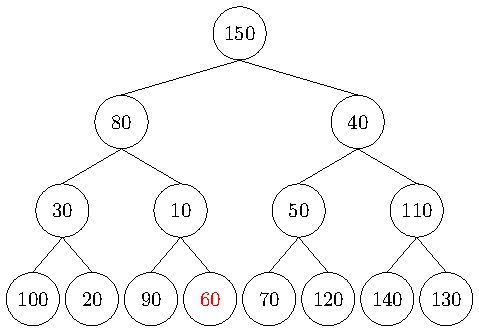
\includegraphics[width=\textwidth]{Figure/Percolate4.pdf}
\end{figure}
\end{minipage}
\end{center}
\begin{center}
\begin{minipage}{0.24\textwidth}
\begin{figure}[H]
  \centering
  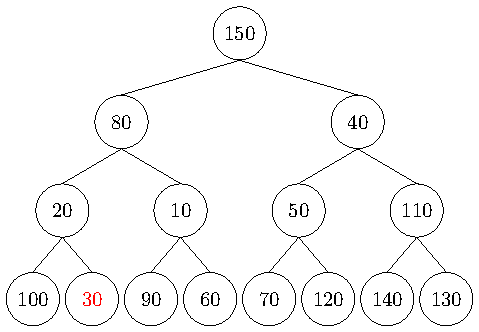
\includegraphics[width=\textwidth]{Figure/Percolate5.pdf}
\end{figure}
\end{minipage}
\begin{minipage}{0.24\textwidth}
\begin{figure}[H]
  \centering
  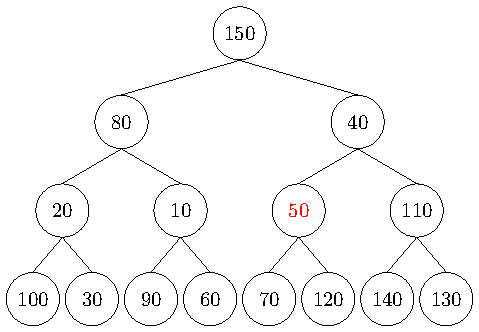
\includegraphics[width=\textwidth]{Figure/Percolate6.pdf}
\end{figure}
\end{minipage}
\begin{minipage}{0.24\textwidth}
\begin{figure}[H]
  \centering
  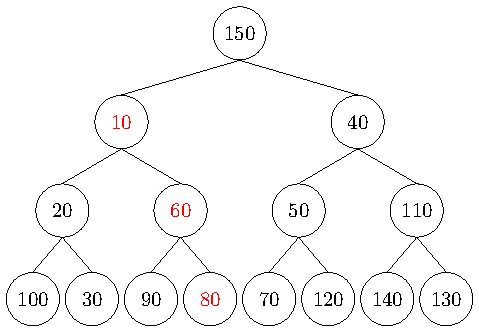
\includegraphics[width=\textwidth]{Figure/Percolate7.pdf}
\end{figure}
\end{minipage}
\begin{minipage}{0.24\textwidth}
\begin{figure}[H]
  \centering
  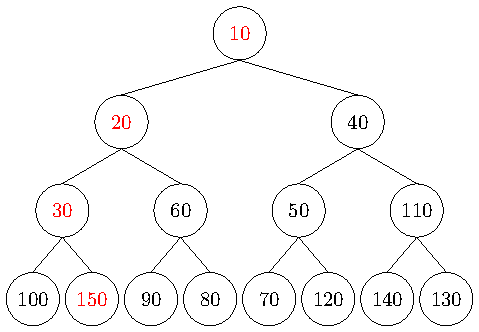
\includegraphics[width=\textwidth]{Figure/Percolate8.pdf}
\end{figure}
\end{minipage}
\end{center}

In this process, we start with the last node that is not a leaf node, compare it with its left and right children, and interchange the node with the larger of its two children. We continue this process with the node until it becomes a leaf node or until the heap property is restored.

To perform a \(k\)-selection, we could find the \(k\)-th smallest or largest element in a set. To build a heap, the average time complexity is \(O(n)\), and the worst-case time complexity is \(O(n \log n)\). To delete from a heap, the time complexity is \(O(\log n)\). Hence, the total runtime for the \(k\)-selection problem is \(O(m + k \log n)\).

For small \(k\), the running time is dominated by the heap-building operation, making it \(O(n)\). For larger values of \(k\), the running time is \(O(k \log n)\).

Alternatively, we could build a smaller heap tree of \(k\) elements and then compare the remaining entries against the heap. If the new element is larger, it replaces the root; otherwise, it is discarded. To build a heap of \(k\) elements, the time complexity is \(O(k)\). The time to process each of the remaining elements is \(O(1)\). To test if an element should be added to the heap, we incur an additional \(O(\log k)\) to delete the root and insert the new element if necessary.

Thus, the total time complexity is \(O(k + (n - k) \log k) = O(n \log k)\). This algorithm also provides a bound of \(n \log n\) for finding the median.
